\section{Experiments} \label{sec::tpp_exp}

In this section, we systematically evaluate the techniques presented in this
work on both synthetic and real-world datasets.  Code and datasets are
available at the following repository:
\url{https://github.com/dragonxlwang/crowd_thurstonian}

\subsection{Simulated Study}

\subsubsection{Datasets} In order to test the effectiveness of \tpp{} under
various scenarios, we generate synthetic datasets with the following parameter
settings.

The ground truth relevance scores of a list of documents
$\{s_{l,i}\}_{i=1,2,...}$ for  query $q_l$  are generated from a uniform
distribution $\mathcal{U}[0, 1]$. Two different lengths are investigated:
$5$~(\textsc{Doc5}) and $30$~(\textsc{Doc30}).  Query difficulty $\delta^2_l$ is
generated from a uniform distribution $\mathcal{U}[0, 0.1]$.  To characterize
the variable quality of answers given by crowd workers, we assume that worker
$t_k$'s expertise and truthfulness $\tau_{k,m}$ on domain $m$ falls into one of
the following categories:

\begin{itemize}
\item \textit{Expert}: $\tau_{k,m} = 10$
\item \textit{Average}: $\tau_{k,m} = 5$
\item \textit{Spammer}: $\tau_{k,m} = 1$
\item \textit{Malicious}: $\tau_{k,m} = -10$
\end{itemize}

Three demographic groups are formed by changing the distributions over these
four categories. Let $p$ denote the categorical distribution over
[\textit{expert, average, spammer, malicious}]:

\begin{itemize}
\item \textsc{Demo1}: $p = [0.2, 0.6, 0.1, 0.1]$. This group represents the most
  common case where average workers are dominant.
\item \textsc{Demo2}: $p = [0.2, 0.4, 0.3, 0.1]$. This group has a large
  proportion of spammers that can hurt the annotation quality.
\item \textsc{Demo3}: $p=[0.2, 0.4, 0.1, 0.3]$. The pairwise preferences given
  by this group can be overwhelmingly misleading due to the presence of too many
  malicious workers.
\end{itemize}

In order to simulate the incompleteness of annotations, which in real world
often depends on factors such as time and budget constraints, we introduce a
variable, \emph{sparsity ratio} (\textsc{Sr}), to control the probability that a
pair of documents is judged by a worker.  For example, if there are a list of
$30$ documents, and $\textsc{Sr} = 0.05$, each worker will judge $\frac{30\times
(30-1)}{2} \times 0.05 = 21.75$ randomly selected pairs.

Finally, the following $8$ datasets are generated. Each of them contains $10$
workers, $10$ query domains and $100$ queries:  \textsc{Doc5Sr1.0Demo1,
Doc5Sr0.5Demo1}, \textsc{Doc5Sr0.5Demo2}, \textsc{Doc5Sr0.5Demo3},
\textsc{Doc30Sr0.1Demo1}, \textsc{Doc30Sr0.05Demo1}, \textsc{Doc30Sr0.05Demo2}
and \textsc{Doc30Sr0.05Demo3}.

\subsubsection{Baselines}
We compare the performance of \textsc{Tpp} against the following four baselines:
\begin{itemize}
\item \textsc{TppUniDom}: \tpp{} without modeling query domains, \ie, all
  queries are treated as from one single domain.
\item \textsc{TppUniExp}: \tpp{} without modeling the domain
  expertise/truthfulness of workers, \ie, all workers have the same expertise
  and truthfulness for a given query domain: $\tau_{k_1,m} = \tau_{k_2, m} =
  \tau_m,$ $\forall k_1, k_2$.
\item \textsc{TppUniDiff}: \tpp{} with identical query difficulty, \ie, all
  queries are equally difficult: $\delta_l^2 = 1/Q,~ \forall l$ with some
  constant $Q$.
\item \textsc{CrowdBt}: \textsc{CrowdBt} \cite{chen2013pairwise} is proposed to
  infer the ground truth scores out of pairwise preferences, which extends the
  Bradley-Terry model by taking worker accuracy into consideration.
  Specifically, a ``worker-independent'' pairwise preference between $d_{i_1}$
  and $d_{i_2}$ for $q_l$ is drawn from a Bernoulli distribution. The
  probability of $d_{i_1} \succ d_{i_2}$ is computed by the Sigmoid function:

  \begin{align}
  \sigma( s_{l, i_1} - s_{l, i_2}) =
    \Big( 1 + \exp\big( -\left(s_{l, i_1} - s_{l, i_2}\right) \big) \Big)^{-1}
    \nonumber
  \end{align}

  Once the pairwise preference is drawn, each worker has a certain probability
  (accuracy) to report it truthfully or ``flip'' it. Compared with \tpp{},
  \textsc{CrowdBt} lacks the mechanism to model multiple query domains, thus
  incapable to characterize workers' domain-dependent expertise and
  truthfulness. Furthermore, it simplifies the generation of inconsistent
  annotations as solely a result from worker accuracy.
\end{itemize}

\begin{table*}[t]
\caption{Crowd Pairwise Preferences Binding Performance
          (Kendall's tau Distance)}
\label{tab::sim_binding}
\setlength\tabcolsep{1.5pt}
\begin{center}
\begin{tabular}{c|rl|rl|rl|rl|rl}
\hline \hline
Dataset	&	\multicolumn{2}{c|}{\textsc{Tpp}}
        &	\multicolumn{2}{|c|}{\textsc{TppUniDom}}
        & \multicolumn{2}{|c|}{\textsc{TppUniExp}}
        & \multicolumn{2}{|c}{\textsc{TppUniDiff}}
        & \multicolumn{2}{|c}{\textsc{CrowdBt}} \\ \hline \hline
\textsc{Doc5Sr1.0Demo1}		& $\mathbf{0.386}$	&	$\pm0.031$	&	$0.414$
        &	$\pm0.037$	&	$0.466$	&	$\pm0.023$	&	$0.402$	&	$\pm0.046$
				& $0.468$	&	$\pm0.047$\\
\textsc{Doc5Sr0.5Demo1} 	& $\mathbf{0.574}$	&	$\pm0.067$	&	$0.728$
        &	$\pm0.066$	&	$0.846$	&	$\pm0.080$	&	$0.628$	&	$\pm0.069$
			  & $0.856$	&	$\pm0.028$\\
\textsc{Doc5Sc0.5Demo2} 	& $\mathbf{0.734}$	&	$\pm0.021$	&	$0.852$
        &	$\pm0.033$	&	$0.940$	&	$\pm0.037$	&	$0.754$	&	$\pm0.047$
			  & $0.960$	&	$\pm0.041$\\
\textsc{Doc5Sr0.5Demo3} 	& $1.592$	&	$\pm0.237$	&	$1.760$	&	$\pm0.077$
        &	$2.550$	&	$\pm0.029$	&	$\mathbf{1.540}$	&	$\pm0.288$
			  & $2.990$	&	$\pm0.060$\\ \hline
\textsc{Doc30Sr0.1Demo1} 	& $\mathbf{22.442}$	&	$\pm1.238$	&	$25.636$
        & $\pm0.302$	&	$29.204$&	$\pm0.291$	&	$26.866$&	$\pm0.456$
			  & $24.420$	& $\pm0.906$\\
\textsc{Doc30Sr0.05Demo1} 	& $\mathbf{40.640}$	&	$\pm0.926$	&	$45.498$
        &	$\pm0.408$	&	$45.636$&	$\pm0.178$	&	$47.258$&	$\pm0.959$
			  & $48.820$	& $\pm2.161$\\
\textsc{Doc30Sr0.05Demo2} 	& $\mathbf{61.818}$	&	$\pm2.713$	&	$70.548$
        &	$\pm0.821$	&	$81.782$&	$\pm0.145$	&	$66.488$&	$\pm2.026$
			  & $104.500$	& $\pm2.469$\\
\textsc{Doc30Sr0.05Demo3} 	& $\mathbf{129.156}$	&	$\pm1.892$	&	$139.154$
        &	$\pm0.243$	&	$142.496$&	$\pm0.587$	&	$135.04$&	$\pm1.864$
			  & $153.390$	& $\pm1.031$ \\ \hline\hline
\end{tabular}
\end{center}
\end{table*}%

\subsubsection{Performance Studies}

We test all the methods on synthetic datasets under various parameter settings,
and report Kendall's tau distance~\cite{kendall1938new}  between the inferred
optimal ranking and the ground truth ranking.  Kendall's tau distance is often
used to measure the dissimilarity between two ranked
lists~\cite{klementiev2008unsupervised}, which is computed as the number of
discordant pairs of the two ranked lists. A pair of documents is discordant if
their relative order is reversed in the two rankings.  For example, suppose two
ranked lists of length $5$ are $d_1 \succ d_2 \succ d_3 \succ d_4 \succ d_5$ and
$d_3\succ d_4 \succ d_1 \succ d_2 \succ d_5$. There are in total
$\frac{5(5-1)}{2}=10$ pairs and $4$ of them are discordant: $\{d_1, d_3\}$,
$\{d_1, d_4\}$, $\{d_2, d_3\}$, $\{d_2, d_4\}$,  thus the Kendall's tau distance
is $4$.  A small Kendall's tau distance indicates good performance. We run each
method on every dataset $5$ times and report the mean and standard deviation in
\Cref{tab::sim_binding}.

\noindent\underline{\emph{Overall Performance.}} \textsc{Tpp} outperforms all
other methods in general (the only exception is on \textsc{Doc5Sr0.5Demo3},
where \textsc{TppUniDiff} gives the best result with a small margin).  Among the
three variants of \textsc{Tpp}, \textsc{TppUniExp} has the worst performance in
recovering the ground truth rankings. This justifies the importance of modeling
workers' domain expertise and truthfulness. Compared with \textsc{CrowdBt},
\textsc{Tpp} consistently behaves significantly better, implying that the
assumed generative process provides more flexibility in modeling and better
explains the generation of inconsistent annotations.

\noindent\underline{\emph{Performance on Different Demographic Groups.}}
Spammers and malicious workers have negative effects on all the methods. The
decrease in performance due to malicious workers is  more striking than that due
to spammers.  Nevertheless, the proposed \textsc{Tpp} is more robust in
resisting the attack from malicious workers than the baselines.  Specifically,
we observe that the Kendall's tau has increased by $88.516$ for \textsc{Tpp}
when changing the dataset from \textsc{Doc30Sr0.5Demo1} to
\textsc{Doc30r0.5Demo3}~\footnote{The maximal Kendall's tau distance for
\textsc{Doc30} is $\frac{30(30-1)}{2} = 435$.}, while this number is $93.656$
for \textsc{TppUniDom}, $96.860$ for \textsc{TppUniExp}, and $104.57$ for
\textsc{CrowdBt}. This demonstrates that \textsc{Tpp} does a better job in
recognizing adversarial workers.

\noindent\underline{\emph{Performance \wrt{} Sparsity Ratio.}} Sparser
annotations provide less evidence to infer the ground truth rankings.  It is
observed that the best performance on \textsc{Doc5Sr0.5Demo1}  ($0.574$) is
still much higher (and thus worse) than the worst performance on
\textsc{Doc5Sr1.0Demo1} ($0.468$).  Similar observations are obtained on the
\textsc{Doc30} datasets.

\subsubsection{Query Domain Prediction}

We investigate the  capability of \textsc{Tpp} in distinguishing between queries
from different domains.

\begin{figure}[h!]
	\centering
		\begin{subfigure}[b]{.5\linewidth}
      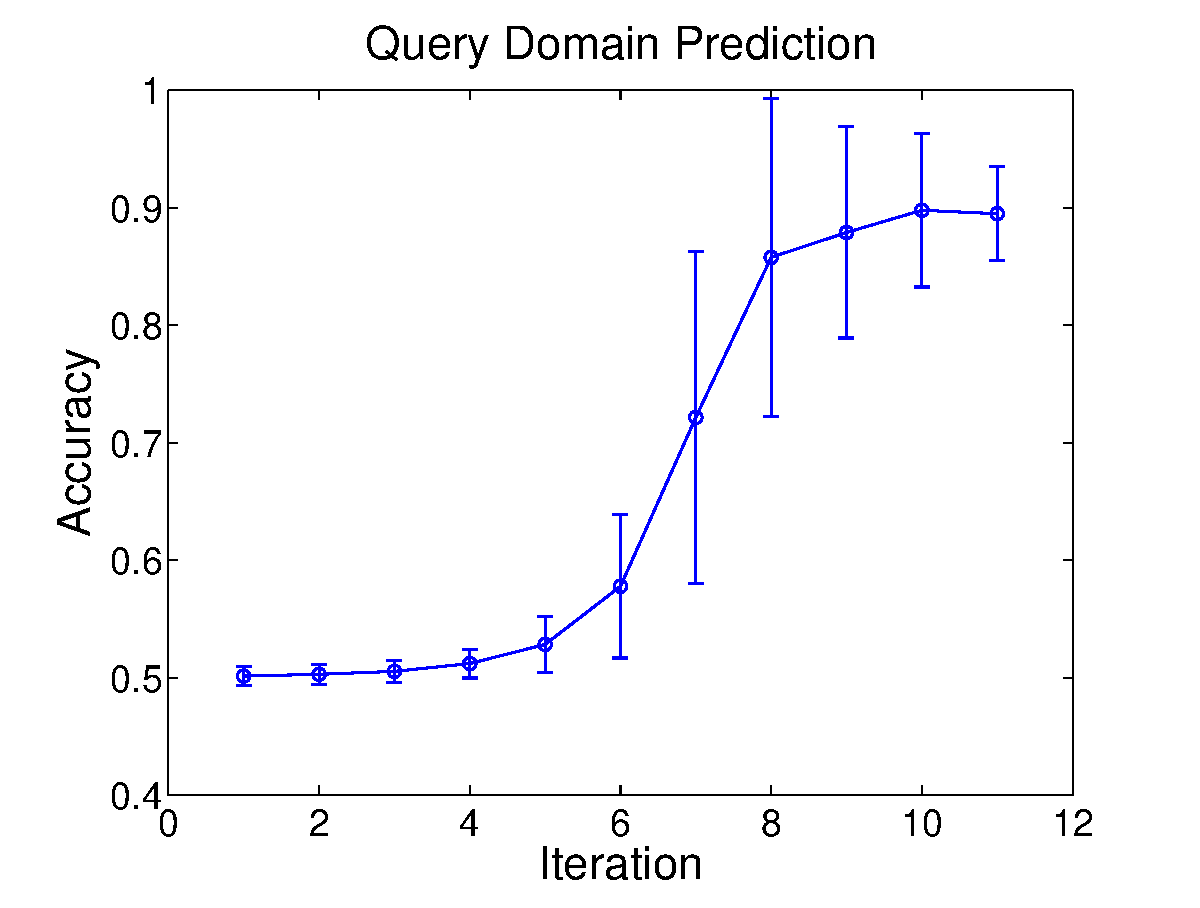
\includegraphics[width=1\textwidth]{crowd-thurstonian/figure/dp_acc.eps}
      \caption{Accuracy} \label{fig::dp_acc}
		\end{subfigure}
    ~
		\begin{subfigure}[b]{.5\linewidth}
      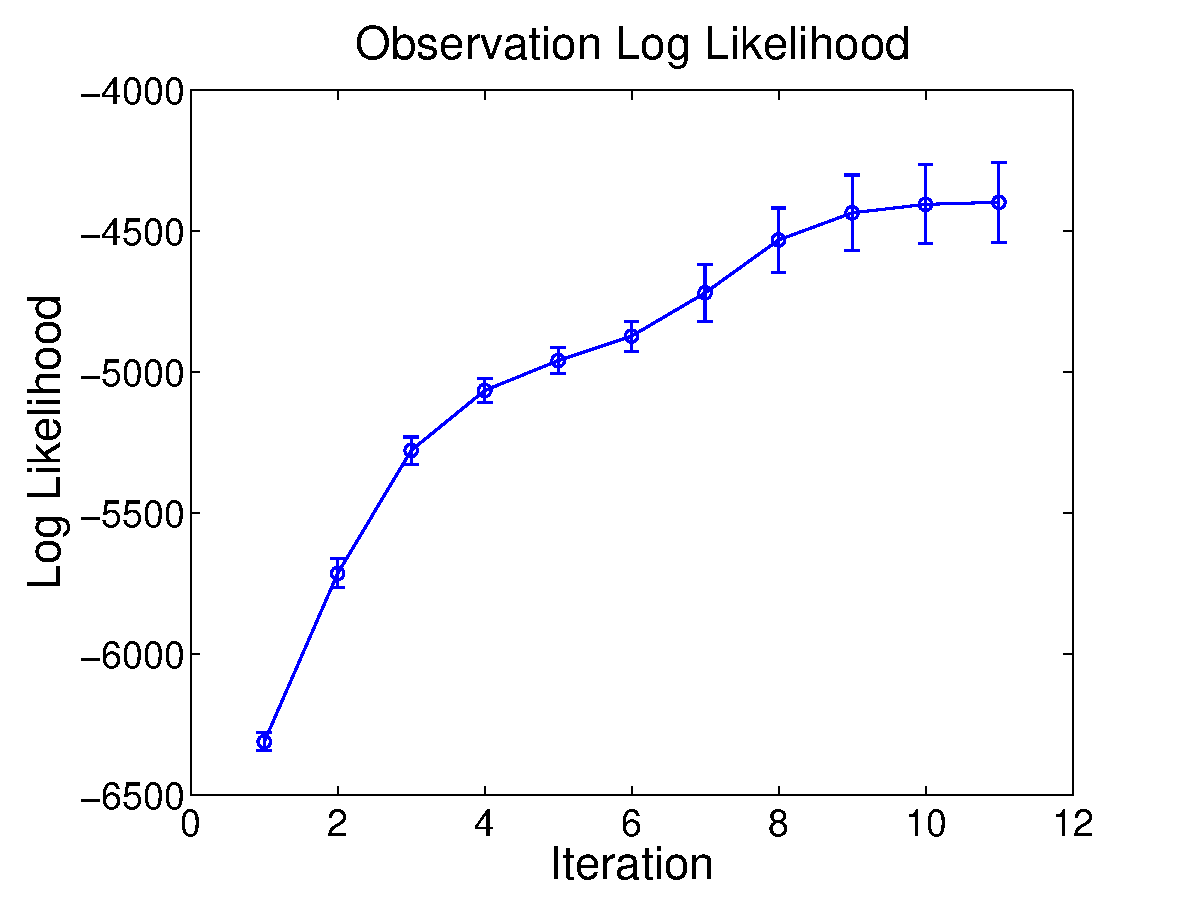
\includegraphics[width=1\textwidth]{crowd-thurstonian/figure/dp_loglikeli.eps}
      \caption{Log Likelihood} \label{fig::dp_loglikeli.eps}
		\end{subfigure}
	\caption{Domain Prediction Accuracy and Model Log Likelihood with Standard Deviations}
  \label{fig::dp}
\end{figure}

We use the setting of \textsc{Doc5Sr0.5Demo1} and generate the pairwise
preferences with only two domains evenly distributed among $100$ queries, for
the ease of illustration.  We run \textsc{Tpp} for $10$ times and plot the
prediction accuracy and the log likelihood. As shown in \Cref{fig::dp},
the algorithm starts from random guess with accuracy around $0.5$, and converges
to an accuracy around $0.895$ in less than $10$ iterations, implying that
\textsc{Tpp} is able to learn query domains effectively and efficiently.

\subsubsection{More Workers but Sparser Annotation}

In practice, when time is the constraining factor, it is plausible to employ a
large number of crowd workers and each worker labels only a few pairs. However,
the situation of \emph{``More Workers but Sparser Annotation''} can potentially
lead to a critical limitation for \tpp{}. On one hand, the number of
parameters $\{\tau_{k,m}\}$ grows with the number of workers. On the other hand,
the amount of data to estimate each $\tau_{k,m}$ decreases.

\begin{table}[h]
  \caption{\textsc{Tpp} Performance with More Workers but Sparser Annotation
  (Kendall's tau Distance)}
\begin{center}
\begin{tabular}{c|rl}
\hline \hline
Dataset	&	\multicolumn{2}{c}{Kendall's tau} \\ \hline \hline
\textsc{Anno100Sr0.01}	& $36.208$	& $\pm0.292$ \\
\textsc{Anno100Sr0.02} 	& $24.328$	& $\pm0.451$ \\
\textsc{Anno200Sr0.01} 	& $25.734$	& $\pm0.394$ \\
\textsc{Anno200Sr0.02} 	& $16.290$	& $\pm0.435$ \\ \hline \hline
\end{tabular}
\end{center}
\label{tab::sparse_anno}
\end{table}%


To evaluate the performance in such scenarios, we create another four datasets
under the setting of \textsc{Doc30Demo1} with more annotators (\textsc{Anno100}
of $100$ annotators and \textsc{Anno200} of $200$ annotators) and lower sparsity
ratios (\textsc{Sr0.01} and \textsc{Sr0.02}).

\begin{figure*}[t!]
    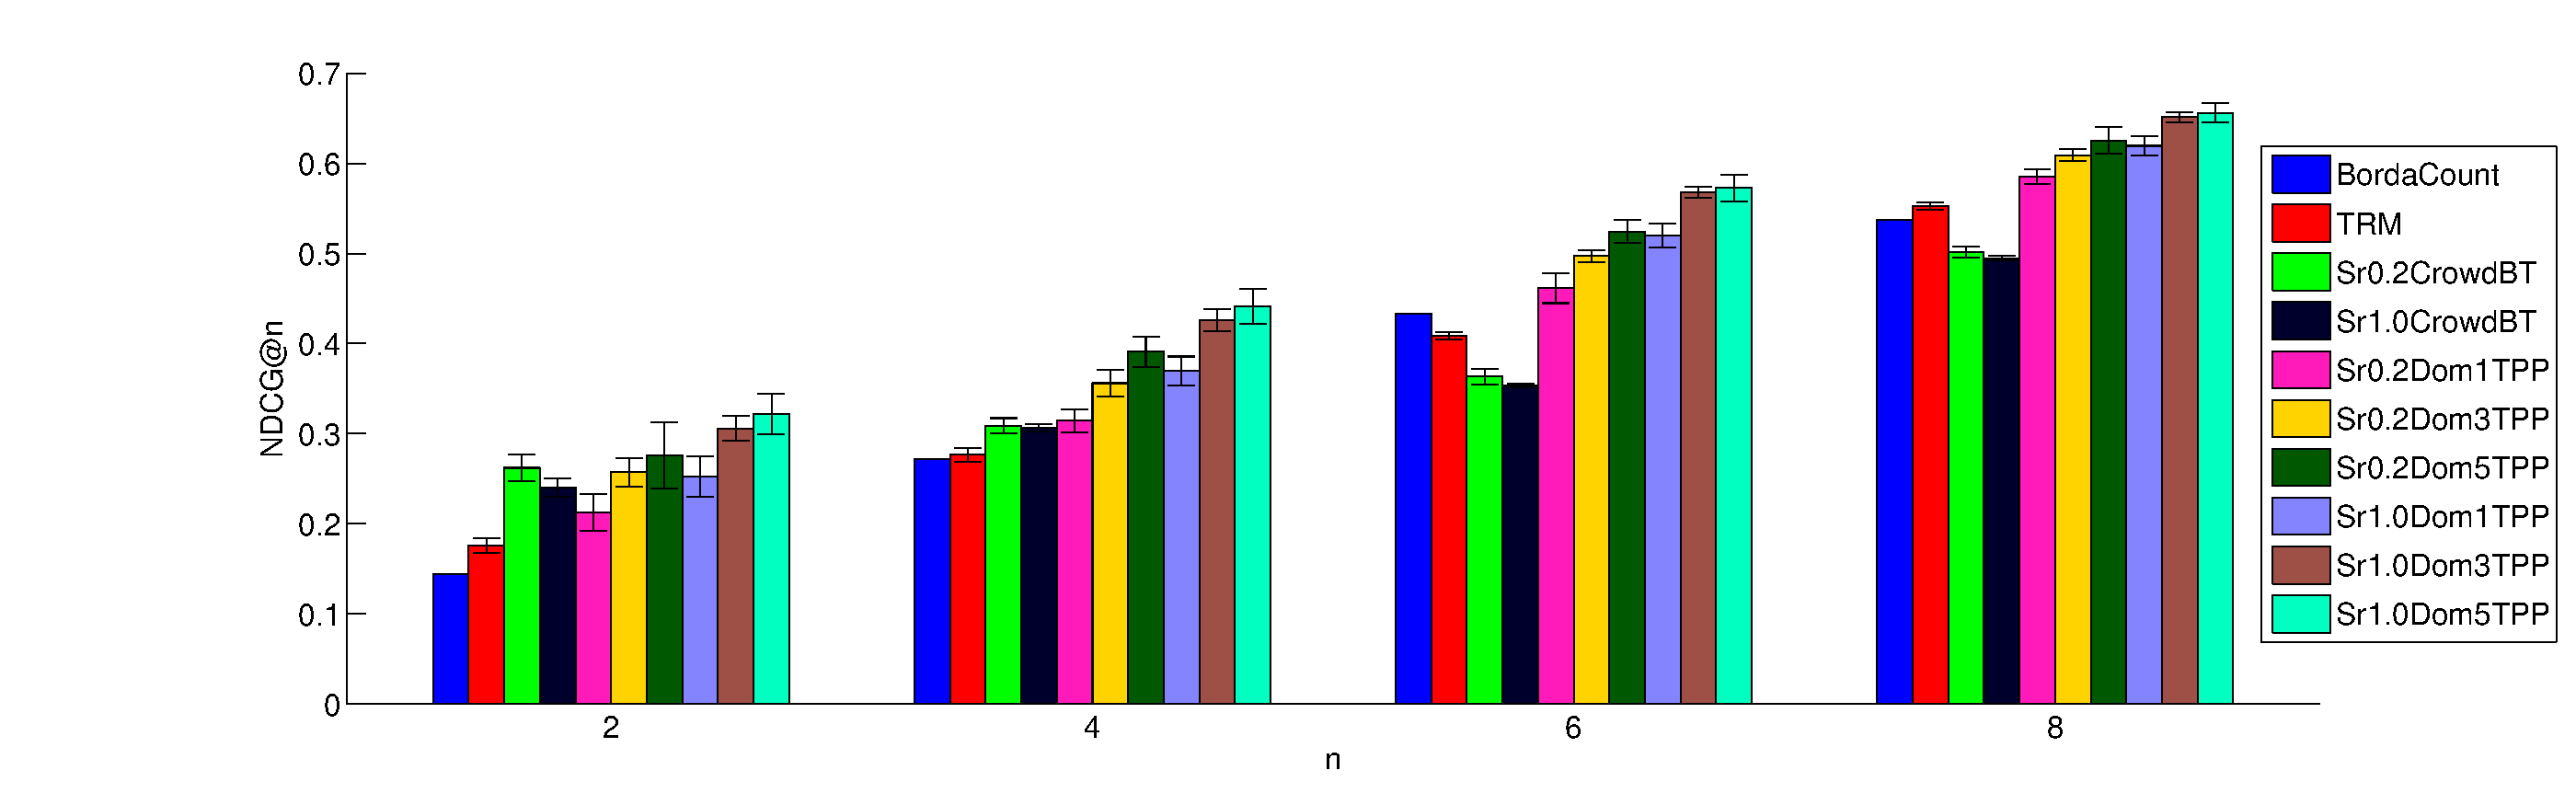
\includegraphics[scale= .4,trim={5cm 0 0 0},clip
      ]{crowd-thurstonian/figure/mq2008_agg.eps}
    \caption{NDCG@n evaluated on MQ2008-agg Dataset}
  \label{fig::mq2008_agg_jet}
\end{figure*}

As shown \Cref{tab::sparse_anno}, the performance of \textsc{Tpp} becomes
worse with ``More Workers but Sparser Annotation'' as Kendall's tau increases
from $22.442$ (\textsc{Doc30Sr0.1Demo1}) to $36.208$ (\textsc{Anno100Sr0.01}).
This is anticipated because the two datasets have the same amount of pairwise
judgements but \textsc{Anno100Sr0.01} involves more workers and has sparser
annotations.  However, \textsc{Anno100Sr0.01} drastically reduces the time cost
and may take only a tenth of the time that \textsc{Doc30Sr0.1Demo1} takes. In
fact, by doubling the number of workers to $200$ or doubling the sparsity ratio
to $0.02$, comparable performance can be achieved with \textsc{Doc30Sr0.1Demo1}.
With an even more aggressive setting \textsc{Anno200Sr0.02} ($20$ times the
number of workers and five times sparser annotations), the performance further
improves. Therefore we conclude that the performance of \tpp{} is reasonably
robust even at the situation of ``more workers and sparser annotation.''


\subsubsection{Malicious Worker Detection} Identifying malicious workers is a
difficult task since the number of malicious workers is usually small so that
the classification is highly imbalanced. We assess the performance of malicious
worker detection by plotting the averaged Receiver Operating Characteristic
(R.O.C.) curves in \Cref{fig::roc}.  In the experiment, with 100 workers
from \textsc{Demo1} and $\textsc{Sr} = 0.01$, \tpp{} performs well with
$\mathrm{AUC}=0.837$ (Area Under the Curve).  When the annotation is
denser~(\textsc{Anno100Sr0.02}),  AUC improves remarkably~($0.924$).  However,
with $200$ workers (\textsc{Demo1}), the difference of AUC between $\textsc{Sr =
0.01}$ and $\textsc{Sr = 0.02}$ is not significant. This can be explained by the
fact that malicious workers are easier to identify in a larger group, even with
sparser annotations.

\begin{figure}[h!]
  \begin{center}
    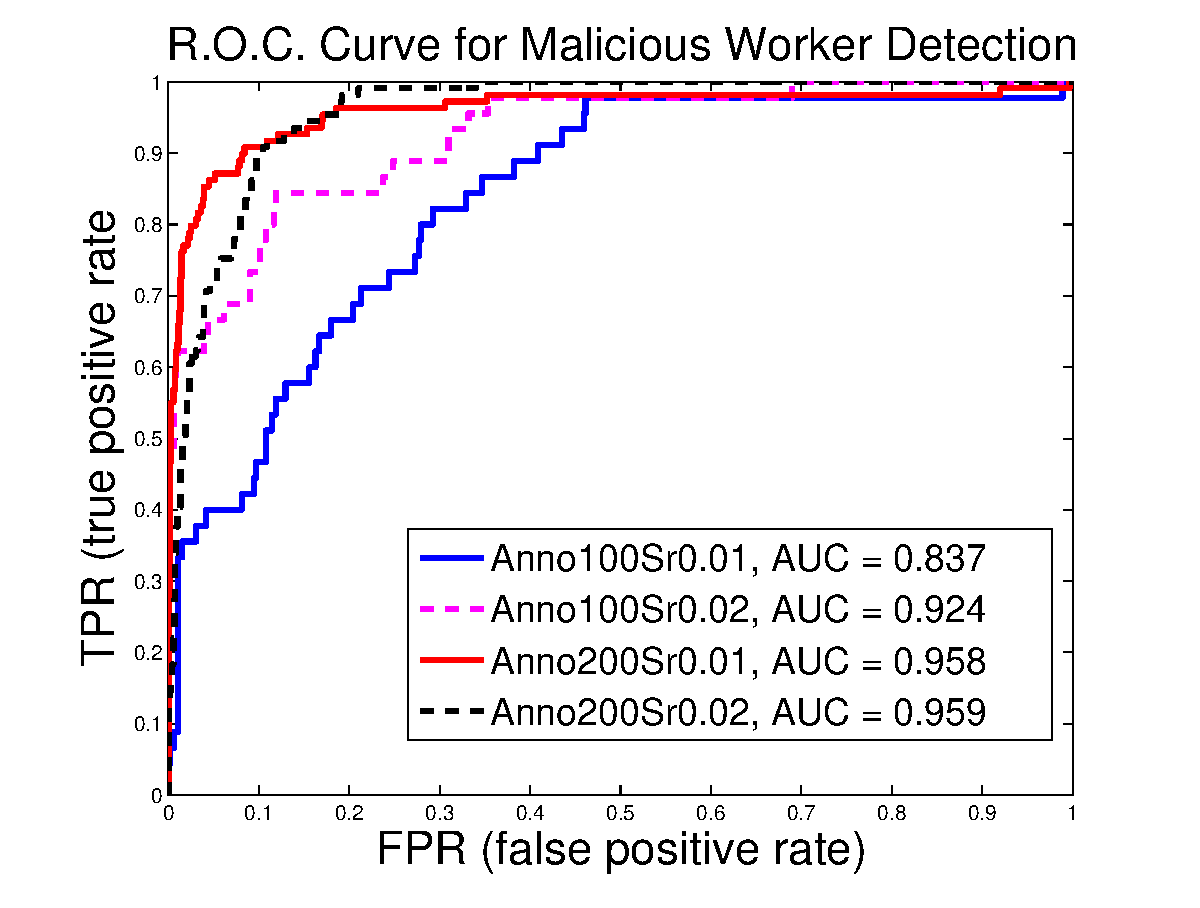
\includegraphics[scale= .50]{crowd-thurstonian/figure/roc.eps}
  \end{center}
  \caption{R.O.C. Curve for Malicious Worker Detection}\label{fig::roc}
\end{figure}

\subsection{Experiments on Real-World Data}

To validate our proposed strategy of binding pairwise preferences into rankings,
we utilize a real-world benchmark MQ2008-agg (part of LETOR
4.0\footnote{http://research.microsoft.com/en-us/um/beijing/projects/letor})
which is originally devised for the rank aggregation~(meta-ranking) task.  The
MQ2008-agg dataset consists of ranked lists from $25$ retrieval systems
(workers). Each document is labeled as \textit{highly relevant}~(2),
\textit{relevant}~(1) or \textit{irrelevant}~(0).  For rank aggregation
algorithms (\trm{} and BordaCount), ranked lists generated from each retrieval
system are taken as input to infer the true ranked list for each query. The
pairwise preference binding algorithms~(\textsc{Tpp} and \textsc{CrowdBt}), on
the other hand, estimate the true ranking out of the pairwise judgements from
each retrieval system (``worker''). The pairwise judgements are randomly sampled
with a sparsity ratio \textsc{Sr}.  In the experiment, we use sparsity ratios
$\textsc{Sr = 1.0}$ (all pairwise judgements are observed) and $\textsc{Sr =
0.2}$.  We evaluate \textsc{Tpp} with 1, 3 and 5 domains. The performance is
compared against both the pairwise preference binding algorithm
\textsc{CrowdBt}, and the rank aggregation algorithms
BordaCount~\cite{aslam2001models} and \textsc{Trm}~(see
\Cref{sec::tpp_trm} and \Cref{app::trm}). In particular,
Bordacount is a simple yet robust algorithm which is essentially a ranking
version of \emph{majority voting}. It infers the true ranking by averaging the
rank positions from each worker.  The performance is measured by NDCG
(Normalized Discounted Cumulative Gain) \cite{jarvelin2000ir}. We use NDCG@$n$
where $n = 2, 4, 6, 8$.

The results are presented in \Cref{fig::mq2008_agg_jet}. In general,
similar performances are observed for the two rank aggregation algorithms with
\textsc{Trm} slightly outperforming Bordacount. With \textsc{Sr1.0},
\textsc{Tpp} and \textsc{CrowdBt} have the same amount of information from
observations as the rank aggregation counterparts. However,
\textsc{Sr1.0CrowdBt} performs better than \textsc{Trm} and Bordacount only at
NDCG@2 and NDCG@4, while it gets worse at NDCG@6 and NDCG@8. In contrast, \tpp{}
consistently outperforms all the baselines, with better performance achieved if
more domains are incorporated.

When the available  annotations become sparser (\textsc{Sr0.2}), the performance
of both \textsc{Tpp} and \textsc{CrowdBt} become worse: NDCGs decrease across
different settings. However, \textsc{Tpp} still significantly outperforms
\textsc{CrowdBt} even with a single domain. In addition, it also outperforms
\textsc{Trm} and Bordacount although the annotation is incomplete. This is
because that the flexible generative process of \textsc{Tpp} properly resolves
the inconsistency from multiple sources.

